\documentclass{article}
\usepackage{polski}
\usepackage{babel}
\usepackage{graphicx}
\usepackage[margin=1in]{geometry}
\usepackage[utf8]{inputenc}
\usepackage{amsmath}
\usepackage{polski}
\usepackage{babel}
\usepackage{hyperref}
\usepackage{graphicx}
\renewcommand{\figurename}{Wykres}
\title{\vspace{4cm} \textbf{Projekt z \\ Projektowania Efektywnych Algorytmów}}
\author{Jakub Grelowski - 262754 \\
        grupa K00-58e \\
        środa - 11:15}
\date{18 stycznia 2022}

\begin{document}

\maketitle

\begin{center}

\large prowadzący: dr inż. Jarosław Mierzwa 

\vspace{1cm}

\Large \textbf{\textit{Zadanie projektowe nr 3 \\ \vspace{1cm} Rozwiązanie problemu komiwojażera za pomocą algorytmu genetycznego}}     
\end{center}

\vspace{1cm}

\newpage

\tableofcontents

\newpage
\section{Wstęp}
\subsection{Cel projektu}
Celem projektu było napisanie programu umożliwiającego analizę efektywności algorytmów genetycznych rozwiązujących asymetryczny problem komiwojażera. 

\subsection{Sposób przechowywania grafów}
\begin{itemize}
    \item Macierz incydencji
\end{itemize}
\subsection{Testowany algorytm}
\begin{itemize}
    \item Algorytm genetyczny
\end{itemize}
\subsection{Rodzaje mutacji}
\begin{itemize}
    \item Transpozycja
    \item Odwracanie
\end{itemize}
\subsection{Metody krzyżowania}
\begin{itemize}
    \item OX - Order crossover
\end{itemize}

\subsection{Implementacja}
Do wykonania projektu wykorzystany został język C\# oraz środowisko programistyczne .NET Framework w wersji 4.8.

\section{Problem komiwojażera}
Problem komiwojażera to problem obliczeniowy polegający na znalezieniu w grafie cyklu Hamiltona o najmniejszej wadze. Cykl Hamiltona to taki cykl, w którym każdy wierzchołek pojawia się dokładnie raz. 

\subsection{Asymetryczny problem komiwojażera}
Kiedy przeszukiwany graf jest skierowany - czyli waga ścieżki z punktu $A$ do punktu $B$ jest taka sama jak waga ścieżki z punktu $B$ do punktu $A$
 - mówimy wtedy o symetrycznym problemie komiwojażera. Tematem projektu jest jednak asymetryczny problem komiwojażera, czyli sytuacja przeciwna - waga ścieżki z punktu $A$ do punktu $B$ nie jest równa wadze ścieżki z punktu B do punktu A.

\newpage
\section{Algorytm genetyczny}
Algorytm genetyczny jest metodą rozwiązywania problemu komiwojażera, polegającą na symulowaniu działania procesu ewolucyjnego. W algorytmie tym, rozwiązania reprezentowane są przez tzw. chromosomy (np. permutacje miast), a ich jakość jest oceniana przez funkcję celu (np. długość trasy).

\subsection{Opis krokowy}
\begin{enumerate}
    \item Inicjalizacja populacji - losowo generowane są początkowe rozwiązania
    \item Ocena jakości rozwiązań - na podstawie funkcji celu (waga ścieżki) oceniana jest jakość każdego chromosomu
    \item Selekcja - na podstawie ocen jakości wybierane są najlepsze rozwiązania, które przechodzą do kolejnej generacji
    \item Krzyżowanie - wybrane rozwiązania są krzyżowane ze sobą, tworząc nowe chromosomy
    \item Mutacja - losowe zmiany w chromosomach, mające na celu wprowadzenie nowych cech
    \item Powtarzaj kroki 2-5 aż nie zajdzie własność stopu (ograniczenie czasowe)
\end{enumerate}

\subsection{Selekcja}
Wykorzystana selekcja losowo wybiera dwa chromosomy i wybiera najlepszy z nich do kolejnej generacji.

\subsection{Krzyżowanie}
Order Crossover (OX) polega na losowym wyborze dwóch fragmentów (podciągów) z jednego chromosomu rodzica, a następnie składaniu ich w nowy chromosom potomny.

\begin{enumerate}
    \item Losowo wybierane są dwa punkty cięcia na chromosomach rodziców, tworząc dwa fragmenty chromosomów.
    \item Z pierwszego chromosomu rodzica kopiuje się fragment pomiędzy punktami cięcia i umieszcza go w odpowiedniej pozycji na chromosomie potomnym.
    \item Następnie reszta genów na chromosomie potomnym jest uzupełniana genami z drugiego chromosomu rodzica, w takiej kolejności w jakiej się na nim pojawiają.
\end{enumerate}

\subsection{Mutacja}
W algorytmie genetycznym mutacja jest procesem, który ma na celu wprowadzenie nowych cech do chromosomów, co pozwala na poszukiwanie nowych rozwiązań i zwiększanie szansy na znalezienie optymalnego rozwiązania.
\begin{itemize}
    \item Transpozycja: polega na losowym wyborze dwóch genów na chromosomie i ich zamianie miejscami
    \item Odwracanie: polega na losowym wyborze dwóch punktów cięcia na chromosomie, a następnie odwróceniu kolejności genów pomiędzy tymi punktami.
\end{itemize}

\newpage
\section{Implementacja}

By zaimplementować różne metody mutacji, całość logiki algorytmu zaimplementowano w abstrakcyjnej klasie \textit{Genetic}. Następnie utworzono konkretne implementacje tej klasy, takie jak \textit{GeneticInverseMutation}, przesłaniające abstrakcyjną metodę \textit{Mutate()}.


\subsection{Najważniejsze klasy w programie}
\begin{itemize}
    \item \textit{Genetic} - abstrakcyjna klasa przechowująca większość logiki.
    \item \textit{GeneticInverseMutation} - implementacja \textit{Genetic} implementująca odwracanie pozycji.
    \item \textit{GeneticTranspositionMutation} - implementacja \textit{Genetic} implementująca zamianę pozycjami.
    \item \textit{Graph} - klasa przechowująca graf w postaci macierzy sąsiedztw oraz jego rozmiar.
    \item \textit{GraphFactory} - klasa generująca losowy graf bądź ładująca graf z pliku tekstowego.
\end{itemize}

\section{Pomiary błędu względnego}
\subsection{W zależności od czasu}
\subsubsection{ftv47.atsp}
\begin{figure}[h!]
\centering
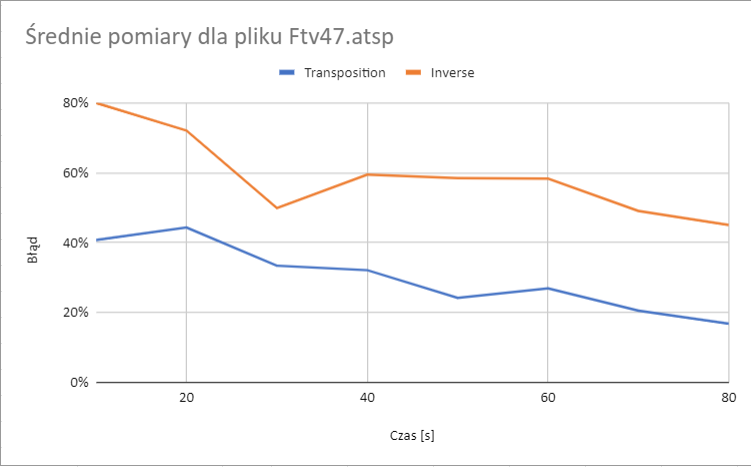
\includegraphics[width=\textwidth]{img/47.png}
\caption{Błąd względny w zależności od czasu - graf ftv47.atsp}
\end{figure}
\newpage
\subsubsection{ftv170.atsp}
\begin{figure}[h!]
\centering
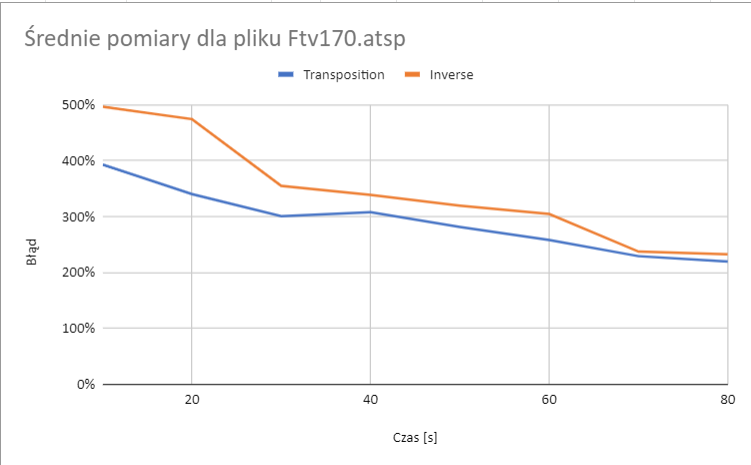
\includegraphics[width=\textwidth]{img/170.png}
\caption{Błąd względny w zależności od czasu - graf ftv170.atsp}
\end{figure}
\newpage
\subsubsection{rgb403.atsp}
\begin{figure}[h!]
\centering
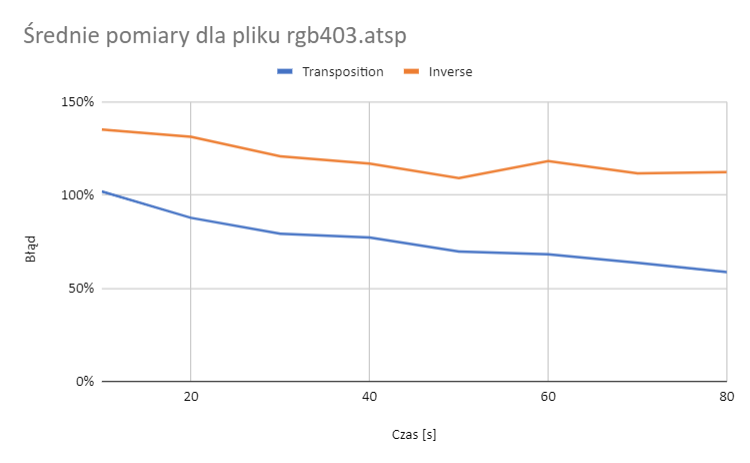
\includegraphics[width=\textwidth]{img/403.png}
\caption{Błąd względny w zależności od czasu - graf rgb403.atsp}
\end{figure}

\newpage
\subsection{W zależności od populacji}
\subsubsection{Transposition}
\begin{figure}[h!]
\centering
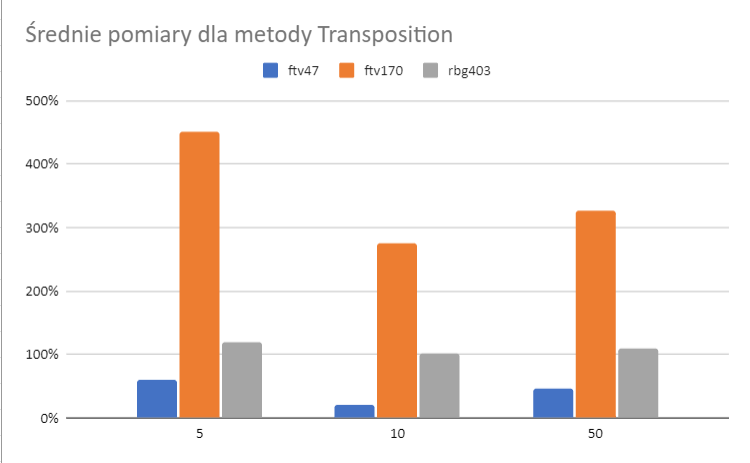
\includegraphics[width=\textwidth]{img/trans.png}
\caption{Błąd względny w zależności od populacji}
\end{figure}
\newpage
\subsubsection{Inverse}
\begin{figure}[h!]
\centering
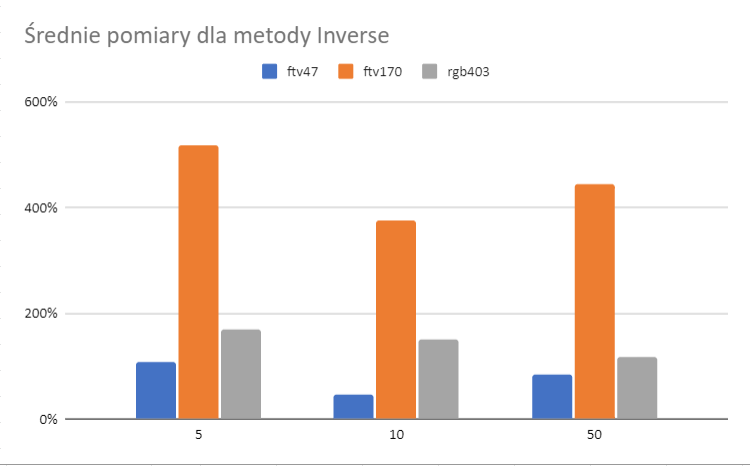
\includegraphics[width=\textwidth]{img/inverse.png}
\caption{Błąd względny w zależności od populacji}
\end{figure}


\section{Porównanie z przeszukiwaniem tabu}
    

\begin{table}[h]
\begin{center}

    \begin{tabular}{r c c}
        graf & tabu search & algorytm genetyczny \\
        ftv47 & 2196 & \textbf{1973} \\
        ftv170 & \textbf{6443} & 8595\\ 
        rgb403 & \textbf{3461} & 4372\\
    \end{tabular}
\end{center}

\end{table}

\section{Wnioski}
Po wynikach pomiarów widoczne jest to, że istotny wpływ na jakość rozwiązań w przypadku algorytmu genetycznego mają parametry początkowe. Średnie pomiary w zależności od populacji pokazują, że dla testowanych algorytmów optymalna populacja znajduje się w okolicach 10 osobników.

\\

Zauważyć można także, że metoda mutacji \textit{Inverse} daje gorsze rezultaty niż metoda \textit{Transposition}. Podobne wyniki dawały analogiczne definicje sąsiedztwa w przeszukiwaniu tabu.  

\\
Porównując rezultaty algorytmu genetycznego z algorytmem tabu widać, 
że algorytm tabu poradził sobie lepiej, jednak nie w każdym przypadku.

\section{Literatura}
\begin{enumerate}
    \item \url{http://www.imio.polsl.pl/Dopobrania/Cw\%20MH\%2007\%20(TSP).pdf}
    \item \url{http://aragorn.pb.bialystok.pl/~wkwedlo/EA5.pdf}
\end{enumerate}


\end{document}
